\documentclass[xcolor=dvipsnames]{beamer}
%
% Choose how your presentation looks.
%
% For more themes, color themes and font themes, see:
% http://deic.uab.es/~iblanes/beamer_gallery/index_by_theme.html
%

\usetheme{Dresden}      % or try Darmstadt, Madrid, Warsaw, Goettingen...
\usecolortheme{beaver}  % or try albatross, beaver, crane, ... seahorse
\usefonttheme{default}  % or try serif, structurebold, ...
\setbeamertemplate{navigation symbols}{}
\setbeamertemplate{section}[numbered]

% Changing the color of itemize item in beamer
\setbeamercolor{enumerate item}{fg=darkred}
\setbeamercolor{itemize item}{fg=darkred}
\setbeamercolor{itemize subitem}{fg=darkred}
\setbeamercolor{description item}{fg=darkred}

% Packages
\usepackage[english]{babel}
\usepackage[utf8x]{inputenc}
\usepackage{multicol}
\usepackage{amsmath,amssymb,amsthm}
\usepackage{amsfonts}
\usepackage{pgfpages}
\usepackage{listings}
% all keywords defined
\lstdefinelanguage[MyLaTeX]{TeX}[LaTeX]{TeX}%
% TeX commands
{moretexcs={enquote,includegraphics,%
part,chapter,section,subsection,paragraph,subparagraph%
tableofcontents,listoffigures,listoftables,maketitle,%
subsection,subsubsection,paragraph,autoref,it,%
textcolor,colorbox,xdefinecolor,colorlet,foreach,%
rowcolors,rowcolor,lstdefinestyle,lstset,KOMAoptions,%
setkomavar,setkomavar*,opening,closing,encl,%
lehead,cehead,rehead,lefoot,cefoot,refoot,%
lohead,cohead,rohead,lofoot,cofoot,rofoot,%
ohead,chead,ihead,ofoot,cfoot,ifoot,%
areaset,color,%
automark,manualmark,markright,markboth,%
tableofcontents,url,clearscrheadfoot,pagemark,headmark,%
setheadtopline,setkomafont,setheadsepline,setfootsepline,%
setfootbotline,chaptermark,thesection,thechapter,%
thesubsection,subtitle,inst,section*,subsection*,institute,%
chapter*,part*,%
qedhere,usetheme,useinnertheme,useoutertheme,usecolortheme,%
,uncover,only,alert,invisible,onslide,mode,mode*,usetikzlibrary,%
draw,filldraw,path,node,usefonttheme,setbeamertemplate,%
declaretheorem,FiveFlowerOpen,%
frontmatter,mainmatter,appendix,backmatter,%
operatorname, titlegraphic, AtBeginSection},%
% LaTeX environments
morekeywords={[2]lstlisting,document,letter,center,flushleft,%
flushright,align,itemize,enumerate,description,tabular,%
titlepage,figure,table,frame,tikzpicture,quote,quotation,verse, 
columns, column, theorem, block},%
% other things (like packages) to highlight
morekeywords={[3]listings,textcomp,courier,xcolor,scrartcl,%
scrlttr2,inputenc,babel,pause,%
fontenc,lmodern,mathptmx,%
helvet,geometry,scrpage2,scrreprt,scrbook,%
article,report,book,hyperref,%
csquotes,amsmath,amssymb,la,beamer,beamerarticle,%
tikz,amsthm,thmtools},
alsoletter={0123456789*},
morekeywords={[4]Optionen},
alsoletter={0123456789*}
}%

%% ------ Colors ------
\definecolor{CadetBlue}{rgb}{.37, .62, .63}
\definecolor{Gray}{rgb}{.70, .70, .70}
\colorlet{maincolor}{orange}
\colorlet{alertedcolor}{red}
\colorlet{examplecolor}{green!50!black}
\colorlet{texicon}{examplecolor}
\colorlet{pdficon}{maincolor}
\colorlet{auxicon}{-examplecolor}
\colorlet{logicon}{black}
\colorlet{bblicon}{-maincolor}
\colorlet{bibicon}{alertedcolor}
\colorlet{texcs}{violet!70}


%% ----- Listings -----
\lstset{ %
basicstyle=\footnotesize\fontfamily{pcr}\selectfont,        % the size of the fonts that are used for the code
backgroundcolor=\color{maincolor!10},             % select a background color
breakatwhitespace=false,         % sets if automatic breaks should only happen at whitespace
breaklines=true,                 % sets automatic line breaking
commentstyle=\ttfamily\color{Green}\fontfamily{pcr}\selectfont, % comment style
deletekeywords={...},            % if you want to delete keywords from the given language
extendedchars=true,              % lets you use non-ASCII characters; for 8-bits encodings only, does not work with UTF-8
frame=lines,                     % adds a frame around the code
keepspaces=true,                 % keeps spaces in text, useful for keeping indentation of code (possibly needs columns=flexible)
keywordstyle=\ttfamily\color{Blue}\fontfamily{pcr}\selectfont\bfseries, % keyword style
keywordstyle={[2]\ttfamily\color{Emerald}\fontfamily{pcr}\selectfont\bfseries},
keywordstyle={[3]\ttfamily\color{Orange}\fontfamily{pcr}\selectfont\bfseries},
keywordstyle={[4]\ttfamily\color{red}\fontfamily{pcr}\selectfont\bfseries},
identifierstyle=\ttfamily\color{black}\fontfamily{pcr}\selectfont,
numbers=left,                    % where to put the line-numbers; possible values are (none, left, right)
numbersep=5pt,                   % how far the line-numbers are from the code
numberstyle=\tiny\color{Gray}\fontfamily{pcr}\selectfont, % the style that is used for the line-numbers
rulecolor=\color{black},         % if not set, the frame-color may be changed on line-breaks within not-black text (e.g. comments (green here))
showspaces=false,                % show spaces everywhere adding particular underscores; it overrides 'showstringspaces'
showstringspaces=false,          % underline spaces within strings only
showtabs=false,                  % show tabs within strings adding particular underscores
stepnumber=1,                    % the step between two line-numbers. If it's 1, each line will be numbered
stringstyle=\ttfamily\color{Gray}\fontfamily{pcr}\selectfont,     % string literal style
tabsize=2                        % sets default tabsize to 2 spaces
}

\lstdefinelanguage{pseudocode}{
keywordstyle=\ttfamily\textbf{\fontfamily{pcr}}\selectfont,
identifierstyle=\ttfamily\color{black}\fontfamily{pcr}\selectfont,
commentstyle=\color{PseudocodeComment}\fontfamily{pcr}\selectfont,
stringstyle=\ttfamily\fontfamily{pcr}\color{PseudocodeString}\selectfont,
%morekeywords={documentclass, usepackage, begin, end, frame},
morecomment=[l]{//},
morecomment=[s]{/*}{*/},
morestring=[b]",
sensitive=false,
showstringspaces=false,
rulecolor=\color{Gray},
escapechar=@,
}

\lstset{
literate={ö}{{\"o}}1
       {Ö}{{\"O}}1
       {ä}{{\"a}}1
       {Ä}{{\"A}}1
       {ü}{{\"u}}1
       {Ü}{{\"U}}1
       {ß}{{\ss}}1
}



\usepackage{xcolor}
\usepackage{framed}

\usepackage{tikz}
\usetikzlibrary{positioning,%
  fit,%
  arrows,%
  automata,%
  trees,%
  intersections,%
  mindmap,%
  shapes.geometric,%
  shapes.arrows,%
  decorations,%
  decorations.pathmorphing,%
  decorations.pathreplacing,%
  matrix,%
  chains,%
  scopes,%
  circuits,%
  circuits.ee.IEC,%
  calc,%
  fadings,%
  lindenmayersystems,%
  decorations.markings,%
  shadows.blur
}

% those small pics from a sheet
\newcommand*{\icon}[2][2]{%
  \tikz\draw[very thick, line join=round]
    (-.5,.5) -- ++(.7,0) -- ++(.3,-.3) --
    ++(-.3,0) -- ++(0,.3) -- ++(.3,-.3) -- ++(0,-.4)
    \foreach \x in {1,...,#1} {
      -- ++(0,-.2)
    }
    -- ++(-1,0) -- cycle
    (-.5,.2) node[fill, text=white,
      inner sep=2pt, minimum width=8mm, anchor=center] {#2}
    ++ (.1,-.3) -- ++(.8,0) \foreach \x in {1,...,#1} {
      -- ++(0,-.1) -- ++(-.8,0) -- ++(0,-.1) -- ++(.8,0)
    };
}

% Color Definition
\lstdefinelanguage{BibTeX}
{keywords={%
  @article,@book,@collectedbook,@conference,@electronic,@ieeetranbstctl,%
  @inbook,@incollectedbook,@incollection,@injournal,@inproceedings,%
  @manual,@mastersthesis,@misc,@patent,@periodical,@phdthesis,@preamble,%
  @proceedings,@standard,@string,@techreport,@unpublished%
  },
comment=[l][\itshape]{@comment},
morekeywords={[2]author,title,year,publisher,editor,booktitle,journal,series,volume,number,pages,institution,note,howpublished},
 }

\newenvironment{mybib}{%
  \begin{thebibliography}{10}
}{%
  \end{thebibliography}
}

% needed in table
\usepackage{pifont}
\newcommand{\goodmark}{\textcolor{green!50!black}{\Pisymbol{pzd}{52}}}
\newcommand{\badmark}{\textcolor{red}{\Pisymbol{pzd}{56}}}


\lstset{language=[MyLaTeX]{TeX}}
\lstset{columns=fixed}
\lstMakeShortInline[columns=fixed]|

% changes for Blockes
\setbeamertemplate{blocks}[rounded][shadow=true]
\setbeamercolor{block title}{fg=black ,bg=gray!20!bg}
\setbeamercolor{block body}{fg=black ,bg=gray!5!bg}

\setbeamercolor{block title alerted}{fg=darkred,bg=pink}
\setbeamercolor{block body alerted}{fg=black,bg=white}


\title[\LaTeX{} Beamer]{Präsentationen mit \LaTeX{} Beamer}
\author{Anika Oellerich}
\date{11.11.2016 -- MetaNook}


\begin{document}
%======================================================================================
\frame{\titlepage}
%\frame[plain]{\titlepage}
%======================================================================================
\begin{frame}{Überblick}
\tableofcontents[]
\end{frame}
%======================================================================================
\section{Was ist Beamer?}
%======================================================================================
\subsection{Einleitung}
\begin{frame}{Was ist Beamer?}
\begin{itemize}
    \item Dokumentenklasse für \LaTeX{} für die Erzeugung von Präsentationen
    \item Keine eigene und keine graphische Anwendung 
    \item Ist in vielen Distributionen enthalten\newline
      (Es kann direkt losgehen.)
\end{itemize}
\end{frame}
%----------------------------------------------------------------------------------
\subsection{Eigenschaften}
\begin{frame}{Funktionsweise von Beamer}
  \begin{itemize}
    \item Kompilieren wie jedes andere \LaTeX-Dokument auch
    \item Normale \LaTeX-Kommandos funktionieren
    \item Sinnvolles funktionales Aussehen von Vorträgen
    \item Einfaches Ein- und Ausblenden von Seitenteilen
    \item Automatische Gliederungen und Navigationsleisten
    \item Präsentationen im PDF-Format können auf jedem Computer dargestellt werden
  \end{itemize}
\end{frame}
%
\begin{frame}{Beamer vs. PowerPoint I}
\begin{tabular}{rcc}
    Aspekte & Beamer & PowerPoint \\
    Erlernen ohne \LaTeX-Kenntnisse & \badmark\badmark & \goodmark \\
    Objekte frei positionieren & \badmark & \goodmark\goodmark \\
    Grafiken direkt erstellen & \badmark & \goodmark \\
    Einbinden von Multimedia & -- & \goodmark \\
    Arbeitsgeschwindigkeit Anfänger & -- & -- \\
    Arbeitsgeschwindigkeit Profi & \goodmark & \goodmark\\
    Erlernen mit \LaTeX-Kenntnissen & \goodmark & \goodmark
\end{tabular}
\end{frame}
%
\begin{frame}{Beamer vs. PowerPoint II}
\begin{tabular}{rcc}
    Aspekte & Beamer & PowerPoint \\
    Dokumentation & \goodmark & \goodmark \\
    Vorlagenqualität & \goodmark & -- \\
    Typographie & \goodmark & \badmark\badmark \\
    Konsistenz des Aussehens & \goodmark\goodmark & \badmark \\
    Visualisierung des Vortragsaufbaus & \goodmark\goodmark & \badmark \\
    Mathematische Formeln & \goodmark\goodmark & \badmark\badmark \\
    Quelltextdarstellung & \goodmark\goodmark & \badmark\badmark
\end{tabular}
\end{frame}
%======================================================================================
\section{Verwendung von Beamer}
%======================================================================================
\subsection{Folien}
%------------------------------------------------------------------------------------
\begin{frame}[fragile]{Grundsätzlicher Aufbau einer Präsentation}
\lstset{language=[MyLaTeX]{TeX}}
 \begin{lstlisting}[gobble=4]
    \documentclass{beamer}

    \usepackage[utf8]{inputenc}
    \usepackage[T1]{fontenc}
    \usepackage{lmodern}
    \usepackage[ngerman]{babel}

    \begin{document}
      \begin{frame}{Grundsätzlicher Aufbau einer ...}
        Kompilieren wie jedes andere
        \LaTeX-Dokument auch.
      \end{frame}
    \end{document}
 \end{lstlisting}
\end{frame}
%
\begin{frame}{Frame - Umgebung}
\begin{itemize}
\item Ein Beamer-Dokument besteht aus mehreren Frames
\item Jeder Frame kann aus mehreren Slides bestehen
\item Die Umgebung \lstinline-frame- verarbeitet bis zu zwei Parameter in 
gescheiften Klammern {}
\begin{itemize}
    \item Der erste Parameter ist der Titel
    \item Der zweite Parameter ist der Untertitel
\end{itemize}
\item Innerhalb der Umgebung frame wird normaler \LaTeX-Code verwendet
\end{itemize}
\end{frame}
%
\begin{frame}[fragile]{Frame - Umgebung}
\lstset{language=[MyLaTeX]{TeX}}
  \begin{lstlisting}[gobble=4]
    \begin{frame}[Optionen]{Frametitel}{Frameuntertitel}
        ... Inhalt ...
    \end{frame}
  \end{lstlisting}
  
\alt<2>{
\begin{block}{Einige Optionen für Inhalt und Layout}
{\color{red}\textbf{fragile}} -- z.B. für Quellcode-Umgebung\\
{\color{red}\textbf{plain}} -- unterdrückt die Anzeige der Überschrift, Fußzeile und Sidebar\\
{\color{red}\textbf{allowframebreaks}} -- große Texte automatisch auf mehrer Folien verteilen\\
{\color{red}\textbf{label=XXX}} -- definiert Folienname für späteren Aufruf mit \\$\backslash$againframe\{XXX\}
\end{block}
}
{
\begin{block}{Optionen für vertikale Ausrichtung}
{\color{red}\textbf{t}} -- Oben\\
{\color{red}\textbf{c}} -- Mitte (Standard)\\
{\color{red}\textbf{b}} -- Unten\\
{\color{red}\textbf{squeeze}} -- Folie vertikal zusammenziehen um Platz zu sparen
\end{block}
}
\end{frame}
%
\begin{frame}[fragile]{Titelseite}
\begin{lstlisting}[gobble=4]
    \title[Kurztitel]{Titel}
    \subtitle[Kurzuntertitel]{Untertitel}
    \author[Kurznamen der Autoren]{Namen der Autoren}
    \institute[Kurzname]{Institut}
    \date[Kurzdatum]{Datum}
    \titlegraphic{Datei}
\end{lstlisting}
Beispiel:
\begin{lstlisting}[gobble=4]
    \title[\LaTeX{} Beamer]{Präsentationen mit \LaTeX{} Beamer}
    %\subtitle[Kurzuntertitel]{Untertitel}
    \author[A. Oellerich]{Anika Oellerich}
    %\institute[Kurzname]{Institut}
    \date{11.11.2016 -- MetaNook}
    %\titlegraphic{Datei}
\end{lstlisting}
\end{frame}
%
\begin{frame}[fragile]{Titelfolie erzeugen}
\begin{columns}[c]
    \begin{column}{0.36\textwidth}
    \begin{lstlisting}[gobble=4]
    \begin{frame}[plain]
    \titlepage
    \end{frame}
    \end{lstlisting}
    \end{column}
    \pause
    \begin{column}{0.7\textwidth}
        \begin{framed}
        \small
        \titlepage
        \end{framed}
    \end{column}
\end{columns}
\end{frame}
%----------------------------------------------------------------------------------------------
\begin{frame}[fragile]{Gliederung}
\begin{columns}[c]
    \begin{column}{0.5\textwidth}
\begin{lstlisting}[gobble=4]
    \section{Was ist Beamer?}
    \subsection{Eigenschaften}
    
    \begin{frame}[]{}
    \tableofcontents[Optionen]
    \end{frame}
    \end{lstlisting}
\end{column}
\begin{column}{0.5\textwidth}
    \begin{itemize}
        \item \LaTeX{} Befehle verwendbar
        \item Inhaltsverzeichnis wird automatisch erstellt
        \item kann in Layout übernommen werden
        \item losgelöst vom Frametitle
    \end{itemize}
\end{column}
\end{columns}
\end{frame}
%----------------------------------------------------------------------------------------------
\begin{frame}[fragile]{Gliederung}
\begin{itemize}
\item Strukturbefehle außerhalb von \lstinline-frame- normal verwenden
\item \lstinline-\tableofcontents- im \lstinline-frame- setzt das Inhaltsverzeichnis
\item Je nach Theme erscheinen \lstinline-\section- und \lstinline-\subsection- auch in Navigationsleisten
\item \lstinline-\section*- und \lstinline-\subsection*- erscheinen in Navigationsleisten aber nicht im Inhaltsverzeichnis
\end{itemize}
\end{frame}
%----------------------------------------------------------------------------------------------
\begin{frame}[fragile]{Inhaltsverzeichnis}
\begin{lstlisting}[gobble=4]
    \tableofcontents[Optionen]
\end{lstlisting}
\begin{block}{Optionen}
{\color{red}\textbf{currentsection}} -- aktuellen Abschnitt hervorheben (Rest halbtransparent)\\
{\color{red}\textbf{currentsubsection}} -- aktuellen Unterabschnitt hervorheben\\
{\color{red}\textbf{pausesections}} -- schrittweise aufdecken, nach jedem Abschnitt Pause\\
{\color{red}\textbf{pausesubsections}} -- nach jedem Unterabschnitt Pause
\end{block}
\end{frame}
%----------------------------------------------------------------------------------------------
\begin{frame}[fragile]{Inhaltsverzeichnis automatisch wiederholen}
Vor jedem Abschnitt automatisch Inhaltsverzeichnis anzeigen:
\begin{lstlisting}[gobble=4]
    \AtBeginSection[]{
    \begin{frame}
    \tableofcontents[currentsection]
    \end{frame}
    }
\end{lstlisting}
\end{frame}
%----------------------------------------------------------------------------------------------
\subsection{Inhalt}
%----------------------------------------------------------------------------------------------
\begin{frame}[fragile]{columns Umgebung}
  \begin{lstlisting}[gobble=4]
    \begin{frame}{Spalten}
      \begin{columns}
        \begin{column}{.5\textwidth}
          Linke Spalte.\\
          ...Text...
        \end{column}
        \begin{column}{.5\textwidth}
          Rechte Spalte.\\
          ...Text...
        \end{column}
      \end{columns}
    \end{frame}
\end{lstlisting}
\end{frame}
%----------------------------------------------------------------------------------------------
\begin{frame}{Spalten}{Beispiel}
\begin{columns}
\begin{column}{.5\textwidth}
Linke Spalte.\\
...Text...
\end{column}
\begin{column}{.5\textwidth}
Rechte Spalte.\\
...Text...
\end{column}
\end{columns}
\end{frame}
%-------------------------------------------------------------------------------------
\subsection{Form}
%----------------------------------------------------------------------------------------------
\begin{frame}[fragile]{Themes}
\begin{description}[labelwidth=5em]
    \item[Theme]
      \begin{itemize}
        \item geladen durch \lstinline-\usetheme{name}- 
        \item bestimmt die \alert{allgemeine Form} der Präsentation
      \end{itemize}
    \item[Inner Theme]
      \begin{itemize}
        \item geladen durch \lstinline-\useinnertheme{name}- 
        \item bestimmt die \alert{Form des Folieninhalts}
      \end{itemize}
    \item[Outer Theme]
      \begin{itemize}
        \item geladen durch \lstinline-\useoutertheme{name}- 
        \item bestimmt die \alert{Form der Layoutelemente}
      \end{itemize}
    \item[Color Theme]
      \begin{itemize}
        \item geladen durch \lstinline-\usecolortheme{name}- 
        \item bestimmt die \alert{allgemeine Farbe} der Präsentation
      \end{itemize}
\end{description}
\end{frame}
%======================================================================================
\section{\LaTeX{} Beamer für Fortgeschrittene}
%======================================================================================
\subsection{Form}
\begin{frame}[fragile]{Themes Verändern}
\begin{block}{Color Theme}
    \begin{itemize}
    \item \lstinline-\usecolortheme[named=color]{structure}-
    \pause
    \item color = red, green, blue, cyan, magenta, yellow, black, darkgray, gray, lightgray, orange, violet, purple, brown
    \end{itemize}
\end{block}
\pause
\begin{block}{Aufzählung} 
    \begin{itemize}
    \item \lstinline-\setbeamercolor{itemize item}{fg=darkred}-
    \item \lstinline-\setbeamercolor{itemize subitem}{fg=darkred}-
    \end{itemize}
\end{block}
\end{frame}
%----------------------------------------------------------------------------------
\subsection{Overlays}
%----------------------------------------------------------------------------------------------
\begin{frame}[fragile]{Einfache Overlays}
  Kommando \lstinline-\pause- blendet Elemente schrittweise ein.

  \begin{lstlisting}[gobble=4]
    \begin{enumerate}
      \item Ein Sandkorn ist kein Sandhaufen.
        \pause
      \item Sandkörner werden durch Hinzufügen
        eines Sandkorns nicht zum Sandhaufen.
        \pause
      \item Induktiv folgt die Aussage.
    \end{enumerate}
\end{lstlisting}

\begin{enumerate}
  \item Ein Sandkorn ist kein Sandhaufen.
    \pause
  \item Sandkörner werden durch Hinzufügen
    eines Sandkorns nicht zum Sandhaufen.
    \pause
  \item Induktiv folgt die Aussage.
\end{enumerate}
\end{frame}
%----------------------------------------------------------------------------------
\begin{frame}{Overlay-Spezifikationen}
  \begin{Satz}[Sandhaufensatz]
    Es gibt keine Sandhaufen.
  \end{Satz}

  \begin{Beweis}<2->
    \begin{enumerate}
      \item<3-> Ein Sandkorn ist kein Sandhaufen.
      \item<4-> Sandkörner werden durch Hinzufügen
        eines Sandkorns nicht zum Sandhaufen.
      \item Induktiv folgt die Aussage. \qedhere
    \end{enumerate}
  \end{Beweis}

  \onslide<5->

  Der Induktionsbeweis ist
  \alert<6>{falsch}!
\end{frame}
%----------------------------------------------------------------------------------
\begin{frame}[fragile]{Overlay-Spezifikationen}
  \begin{lstlisting}[gobble=4]
    \begin{Satz}[Sandhaufensatz]
      Es gibt keine Sandhaufen.
    \end{Satz}

    \begin{Beweis}<2->
      \begin{enumerate}
        \item<3-> Ein Sandkorn ist kein Sandhaufen.
        \item<4-> Sandkörner werden durch Hinzufügen
          eines Sandkorns nicht zum Sandhaufen.
        \item Induktiv folgt die Aussage. \qedhere
      \end{enumerate}
    \end{Beweis}

    \onslide<5->
    Der Induktionsbeweis ist \alert<6>{falsch}!
  \end{lstlisting}
\end{frame}
%----------------------------------------------------------------------------------
\begin{frame}[fragile]{Ein- und Ausblenden}
  \begin{itemize}
    \item \lstinline|\uncover<2->{Inhalt}| blendet Inhalt erst ab
      Folie~2 ein. Der Platz wird jedoch vorher schon reserviert.
    \item \lstinline|\only<3->{Inhalt}| setzt Inhalt erst ab Folie~3.
      Zuvor wird kein Platz reserviert.
    \item \lstinline|\invisible<4->{\alert <4>{Inhalt}}| Inhalt wird ab Folie~4 verschwinden
  \end{itemize}

  \begin{lstlisting}[gobble=4]
    In diesem \uncover<2->{Satz} werden \only<3->{Worte }
    eingeblendet. 
    \invisible<4->{\alert{Dieser Satz wird verschinden.}}}
  \end{lstlisting}
  \only{In diesem \uncover<2->{Satz} werden
    \only<3->{Worte }eingeblendet. \invisible<4->{\alert{Dieser Satz wird verschinden.}}}
\end{frame}
%----------------------------------------------------------------------------------
\subsection{Erweiterungen}
\begin{frame}[fragile, squeeze]{Artikelfassung}
  \begin{block}{Ziel}
    Generierung von Artikelfassung und Präsentation
    aus demselben Quellen-Dokument.
  \end{block}

  \pause
    \setbeamercolor{block title alert}{bg=lightgray}
    \setbeamercolor{block body alert}{fg= black, bg= white}
  \begin{alertblock}{Problem}
    \begin{tabular}{r@{ }l}
      \textbf{Präsentation} & Dokumentenklasse von Beamer.\\
      \textbf{Artikel} & Dokumentenklasse von KOMA-Script.
    \end{tabular}
  \end{alertblock}

  \pause

  \begin{block}{Lösung}
    \begin{itemize}
      \item Ein \LaTeX-Dokument für den Inhalt.
      \item Zwei \LaTeX-Dokumente für beide Dokumentenklassen.
      \item Einbinden des Inhalts mit \lstinline-\input-.
    \end{itemize}
  \end{block}
\end{frame}
%----------------------------------------------------------------------------------
\begin{frame}[fragile, squeeze]{Einbinden des Inhalts}
\begin{figure}
    \centering

  %\begin{center}
    \begin{tikzpicture}[
        on grid,
        auto,
        node distance=15mm and 35mm,
        engine/.style={
          font=\rmfamily\Large\bfseries,
          inner sep=2pt
        }
      ]

      \node (content tex) {\shortstack{\textcolor{texicon}{\icon{TEX}}\\\texttt{content.tex}}};

      \uncover<2->{
        \node[below left=of content tex] (beamer tex)
          {\shortstack{\textcolor{texicon}{\icon{TEX}}\\\texttt{beamer.tex}}};
        \node[below right=of content tex] (article tex)
          {\shortstack{\textcolor{texicon}{\icon{TEX}}\\\texttt{article.tex}}};
      }

      \uncover<3->{
        \node[below=of beamer tex, engine](make beamer) {\LaTeX.mk};

        \node[below=of article tex, engine](make article) {\LaTeX.mk};

        \node[below=of make beamer] (beamer pdf)
          {\shortstack{\textcolor{pdficon}{\icon{PDF}}\\\texttt{beamer.pdf}}};
        \node[below=of make article] (article pdf)
          {\shortstack{\textcolor{pdficon}{\icon{PDF}}\\\texttt{article.pdf}}};
      }

      \only<2->{
        \draw[very thick]
        (content tex.west) edge[->] node[swap, near start]
          {\texttt{\color{texcs}\bfseries\textbackslash input}} (beamer tex.north);

        \draw[very thick]
          (content tex.east) edge[->] node[near start]
            {\texttt{\color{texcs}\bfseries\textbackslash input}} (article tex.north);
      }

      \only<3->{
        \draw[very thick]
          (beamer tex) edge[->] (make beamer)
          (article tex) edge[->] (make article);

        \draw[very thick]
          (make beamer) edge[->] (beamer pdf)
          (make article) edge[->] (article pdf);
      }
    \end{tikzpicture}
  %\end{center}
  \end{figure}
\end{frame}

\begin{frame}[fragile]{Inhalt \texttt{content.tex}}
  \begin{lstlisting}[gobble=4]
    \title{Mein Vortrag}
    \author{Mein Name}

    \begin{document}
      \begin{frame}
        \maketitle
      \end{frame}

      \begin{frame}{Folientitel}
        Hier passierts \dots
      \end{frame}
    \end{document}
  \end{lstlisting}
\end{frame}
%----------------------------------------------------------------------------------
\begin{frame}[fragile]{Dokumentenklassen}
 Für die Folien \texttt{beamer.tex}
  \begin{lstlisting}[gobble=4]
    % Beamer als Dokumentenklasse verwenden
    \documentclass{beamer}
    % gemeinsamen Inhalt einbinden
    \input{content.tex}
  \end{lstlisting}

  Für den Artikel \texttt{article.tex}
  \begin{lstlisting}[gobble=4]
    % KOMA-Script als Dokumentenklasse verwenden
    \documentclass{scrartcl}
    % Beamer als Paket laden
    \usepackage{beamerarticle}
    % gemeinsamen Inhalt einbinden
    \frame{content.tex}
  \end{lstlisting}
\end{frame}
%----------------------------------------------------------------------------------
\begin{frame}[fragile]{Modes}
  \begin{tabular}{r@{ }l}
    \texttt{presentation} & nur für Folien\\
    \texttt{article} & nur für Artikel\\
    \texttt{all} & für Folien und Artikel (Standard)
  \end{tabular}

  \begin{lstlisting}[gobble=4]
    \mode
    <name>
  \end{lstlisting}
  Wechselt den aktuellen Mode.

  \begin{lstlisting}[gobble=4]
    \mode*
  \end{lstlisting}
  Automatische Modeumschaltung:
  \begin{itemize}
    \item Innerhalb von \lstinline-frame- Mode {all}.
    \item Außerhalb von \lstinline-frame- Mode {article}.
  \end{itemize}
\end{frame}


\subsection{Quellen}
\begin{frame}{GitHub -- Links}
\begin{itemize}
    \item Meine Dateien: \newline 
    \url{https://github.com/anioell/Nook-LaTeX-Beamer}
    \item \LaTeX{} - Arbeiten mit TikZ von Dennis Labitzke \newline
    \url{https://github.com/labitzkedennis/Nook2016-TikZ}
    \item Einführung in \LaTeX{} von Malte Schmitz\newline
    \url{https://github.com/malteschmitz/latex}
\end{itemize}
\end{frame}


\begin{frame}{Zum Weiterlesen}
  \begin{mybib}
    \bibitem{Tantau}
      Till Tantau, Joseph Wright und Vedran Mileti\'c.
      \newblock The \textsc{beamer} \textit{class}, User Guide.
      \newblock \alt<presentation>{\href{http://mirrors.ctan.org/macros/latex/contrib/beamer/doc/beameruserguide.pdf}{\texttt{beameruserguide.pdf}}}{\url{http://mirrors.ctan.org/macros/latex/contrib/beamer/doc/beameruserguide.pdf}}, Oktober 2013.

    \bibitem{Tantau}
      Till Tantau.
      \newblock \emph{Beamer: Strahlende Vorträge mit \LaTeX},
      \newblock Präsentieren und Dokumentieren -- Tools.
      \newblock Vorlesung vom 31. Oktober 2012.
  \end{mybib}
\end{frame}
\end{document}
